\chapter{Resultados y discusi\'on}
\label{ch:resAuger}

\section{C\'alculo de la exposici\'on}
	
	\section{\label{sc:sim_prop_tierra}Propagaci\'on dentro de la tierra}
	
	Para simular la propagaci\'on del \tauon{} en la tierra se utiliz\'o un programa que realiza el c\'alculo mediante m\'etodos de Monte Carlo, desarrollado por J. A. Mu\~niz y E. Zas, del grupo de altas energ\'ias de la Universidad de Santiago de Compostela.
	Una explicaci\'on detallada del programa puede encontrarse en \cite{gap_tau_tierra}.
	
	Este c\'odigo permite propagar los \nutau{}s y \tauon{}s en la tierra y, dado el \'angulo cenital \tita{} y la energ\'ia del neutrino incidente \enu{}, calcular la probabilidad de que un \tauon{} alcance la superficie de la tierra con energ\'ia \etau{}.
	Estos c\'alculos se realizan teniendo en cuenta la interacci\'on del \nutau{} via CC y CN, la p\'erdida de energ\'ia del \tauon{} (con $\beta$\footnote{ver ecuaci\'on \ref{eq:tau_losses}} dependiente o independiente de la energ\'ia) y la regeneraci\'on del flujo de \nutau{} debido a interacciones via CN y a decaimientos de leptones \tauon{}.
	
	La simulaci\'on consta de dos etapas principales que se alternan hasta que se alcanza la superficie:
	
	\begin{description}
	\item[\textbf{Interacci\'on del \nutau{}:}] Se hace interactuar al neutrino siguiendo una distribuci\'on exponencial en $x$, donde $x$ es la variable que mide la cantidad de materia atravesada por el \nutau{}. Para ello, se tienen en cuenta interacciones via CC y CN. Si se diera una interacci\'on via CC, se produce un \tauon{} cuya energ\'ia proviene de muestrear la seccion efic\'az diferencial de CC, $\frac{d\sigma^{cc}}{dy}$. En cambio, si la interacci\'on se produce via CN, es generado un nuevo \nutau{} de energ\'ia menor que se hace interactuar nuevamente.
	\item[\textbf{Propagaci\'on del \tauon{}:}] En caso de que un \tauon{} sea producido, se lo propaga de a peque\~nos pasos, calculando en cada uno de ellos la energ\'ia perdida debido a la interacci\'on con el medio y la probabilidad de decaimiento (como funci\'on de su energ\'ia). Si decayese produciendo un nuevo \nutau{}, se comienza el procedimiento nuevamente desde el punto del \'ultimo decaimiento.
	\end{description}
	
	Este Programa fue validado utilizando programas mucho m\'as complejos, como ANIS \cite{anis}.
	Tambi\'en se realiz\'o una comparaci\'on del flujo de \tauon{} saliente obtenido mediante el calculo te\'orico que puede encontrarse en \cite{prop_tau} y el obtenido por este programa, para diferentes \'angulos cenitales.
	Esta \'ultima comparaci\'on se muestra en la figura \ref{fig:comp_tau_mc_teo}, en la que se observa un muy buen acuerdo entre ambos resultados.
	%
	\begin{figure}[h!]
		\begin{center}
		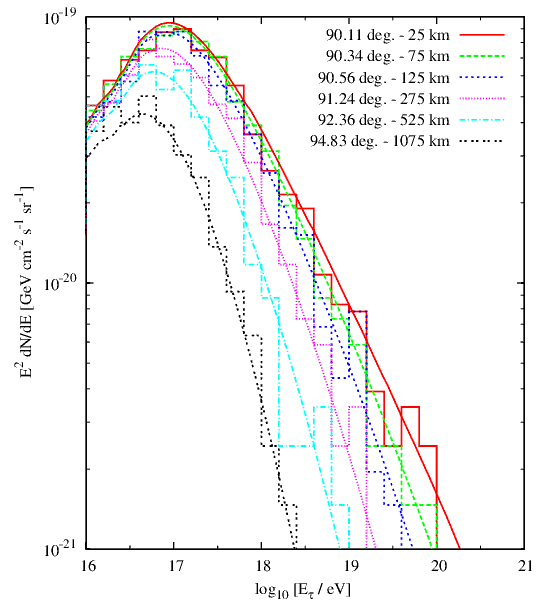
\includegraphics[width=0.75\textwidth]{fig/simulacionAuger/comp_tau_mc_teo}
		\caption{\label{fig:comp_tau_mc_teo} Comparaci\'on de los flujos salientes obtenido anal\'iticamente y mediante simulaci\'on. Los histogramas corresponden a los resultados del Monte Carlo, mientras que la l\'inea llena al c\'alculo te\'orico.}
		\end{center}
	\end{figure}
	
	
	\subsection{Combinaci\'on de los an\'alisis}
	
	\begin{figure}[h!]
		\begin{center}
			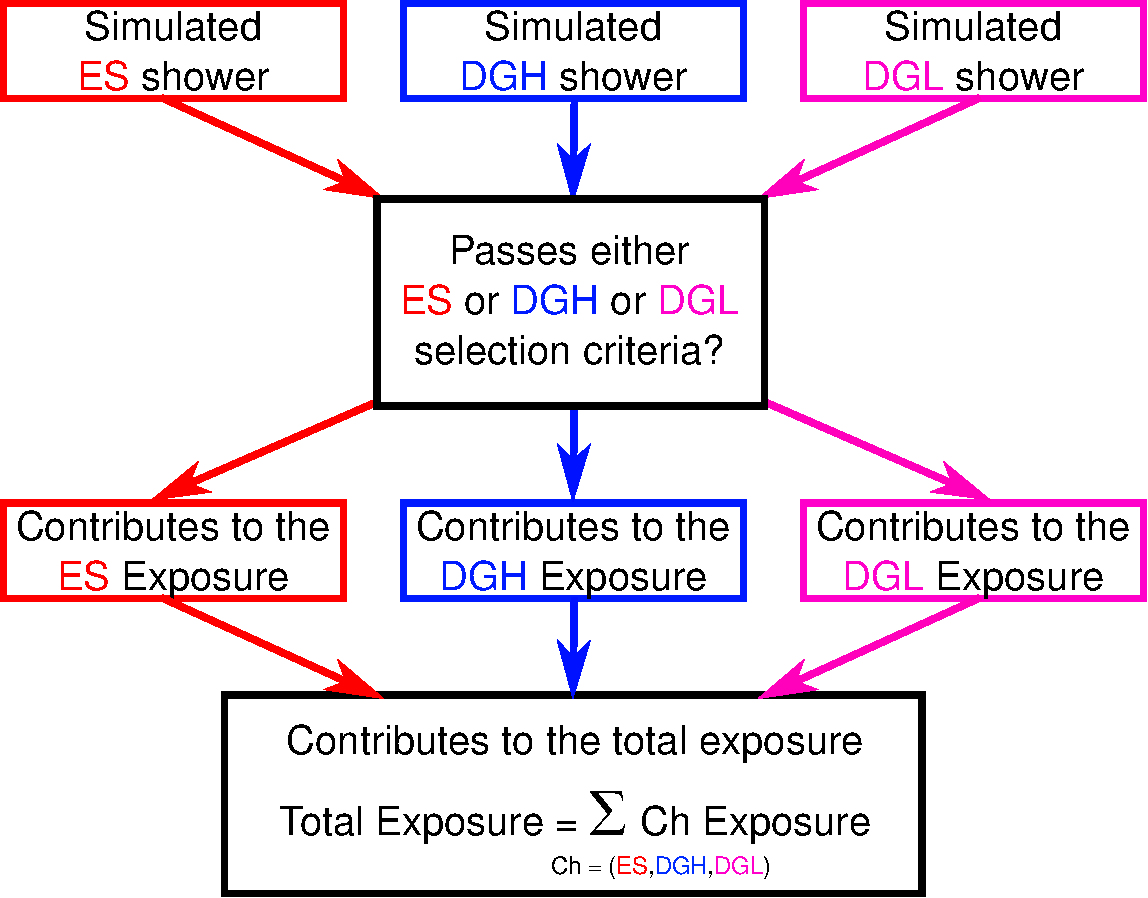
\includegraphics[width=0.9\textwidth]{fig/resultadosAuger/sketch_combined_4}
			\caption{asd}
			\label{fig:}
		\end{center}
	\end{figure}
	
	\begin{figure}[h!]
		\begin{center}
			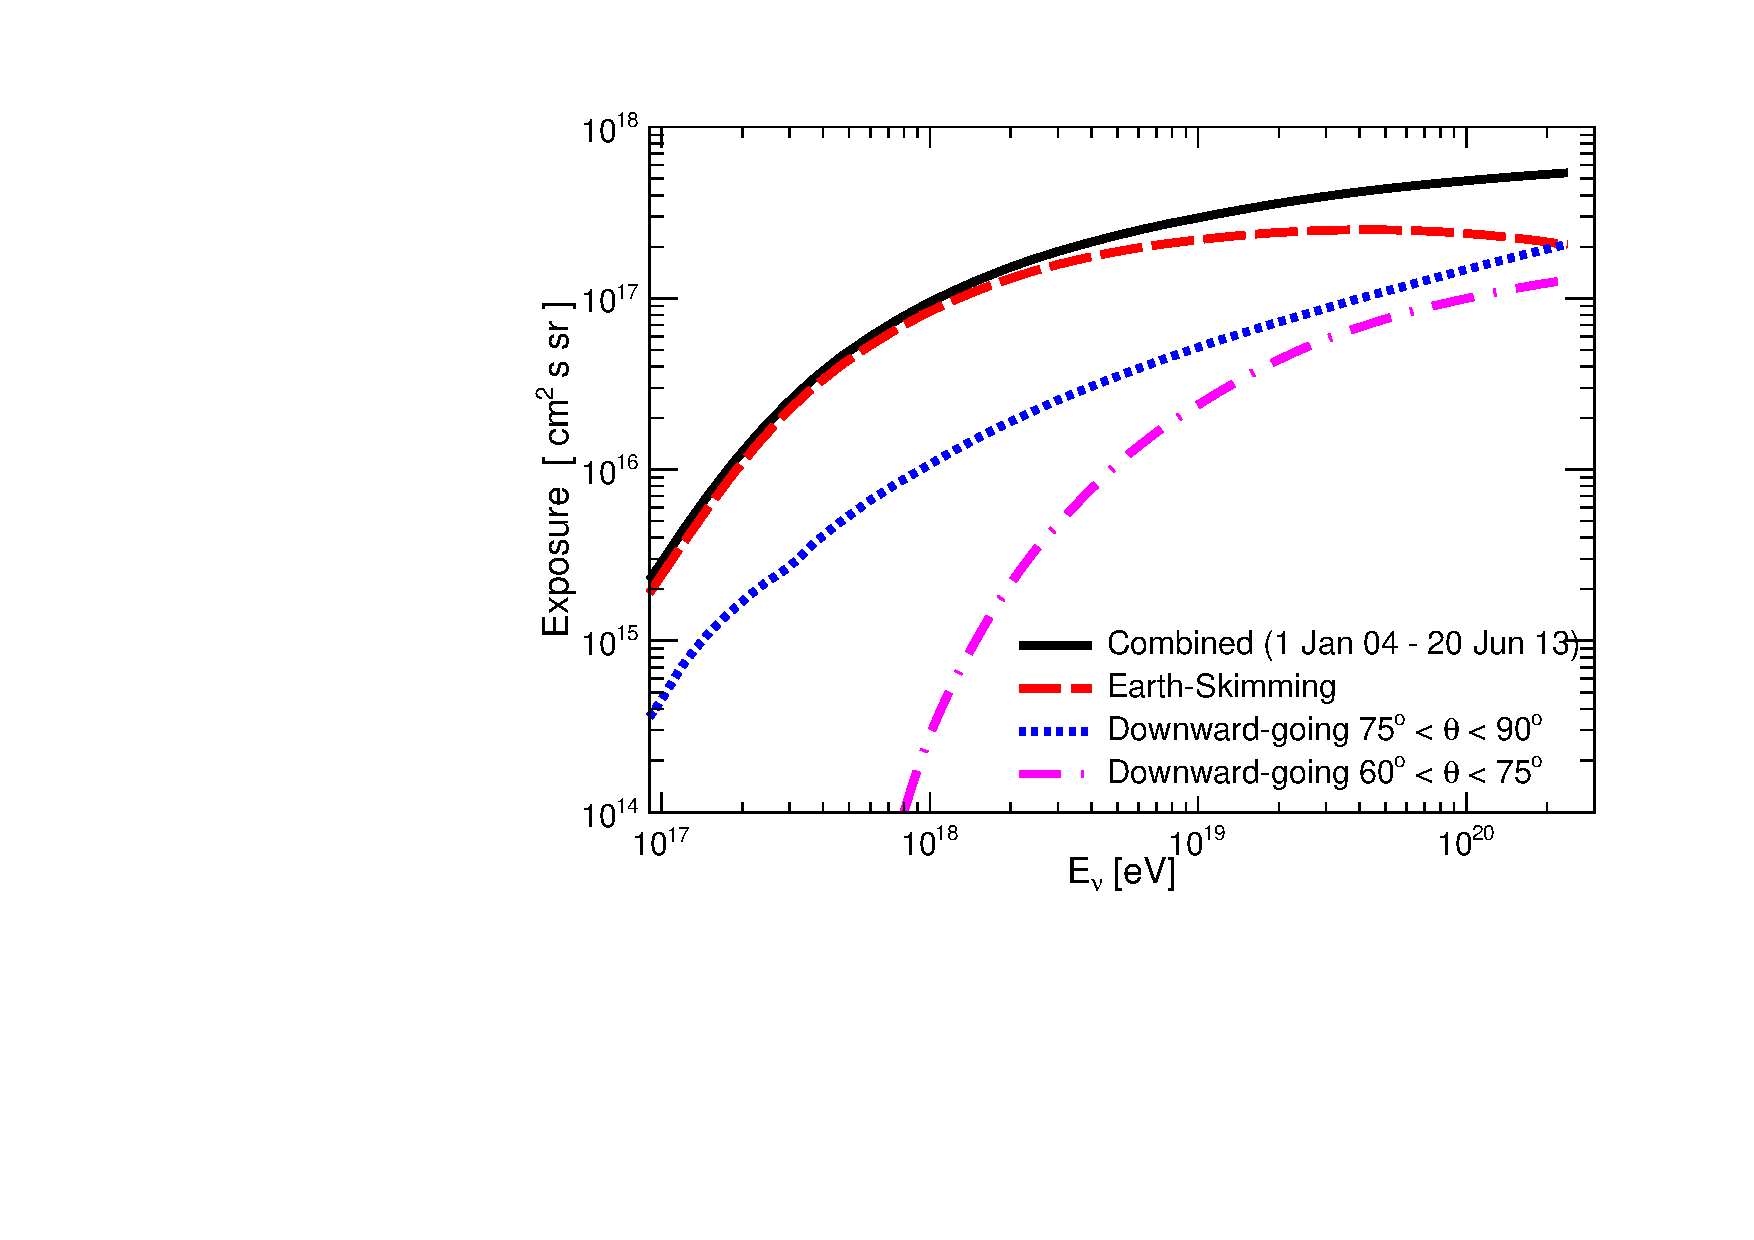
\includegraphics[width=0.9\textwidth]{fig/resultadosAuger/exposure_combined_ageing}
			\caption{asd}
			\label{fig:}
		\end{center}
	\end{figure}

	
	\subsection{Envejecimiento del detector}
	
	\begin{figure}[h!]
		\begin{center}
			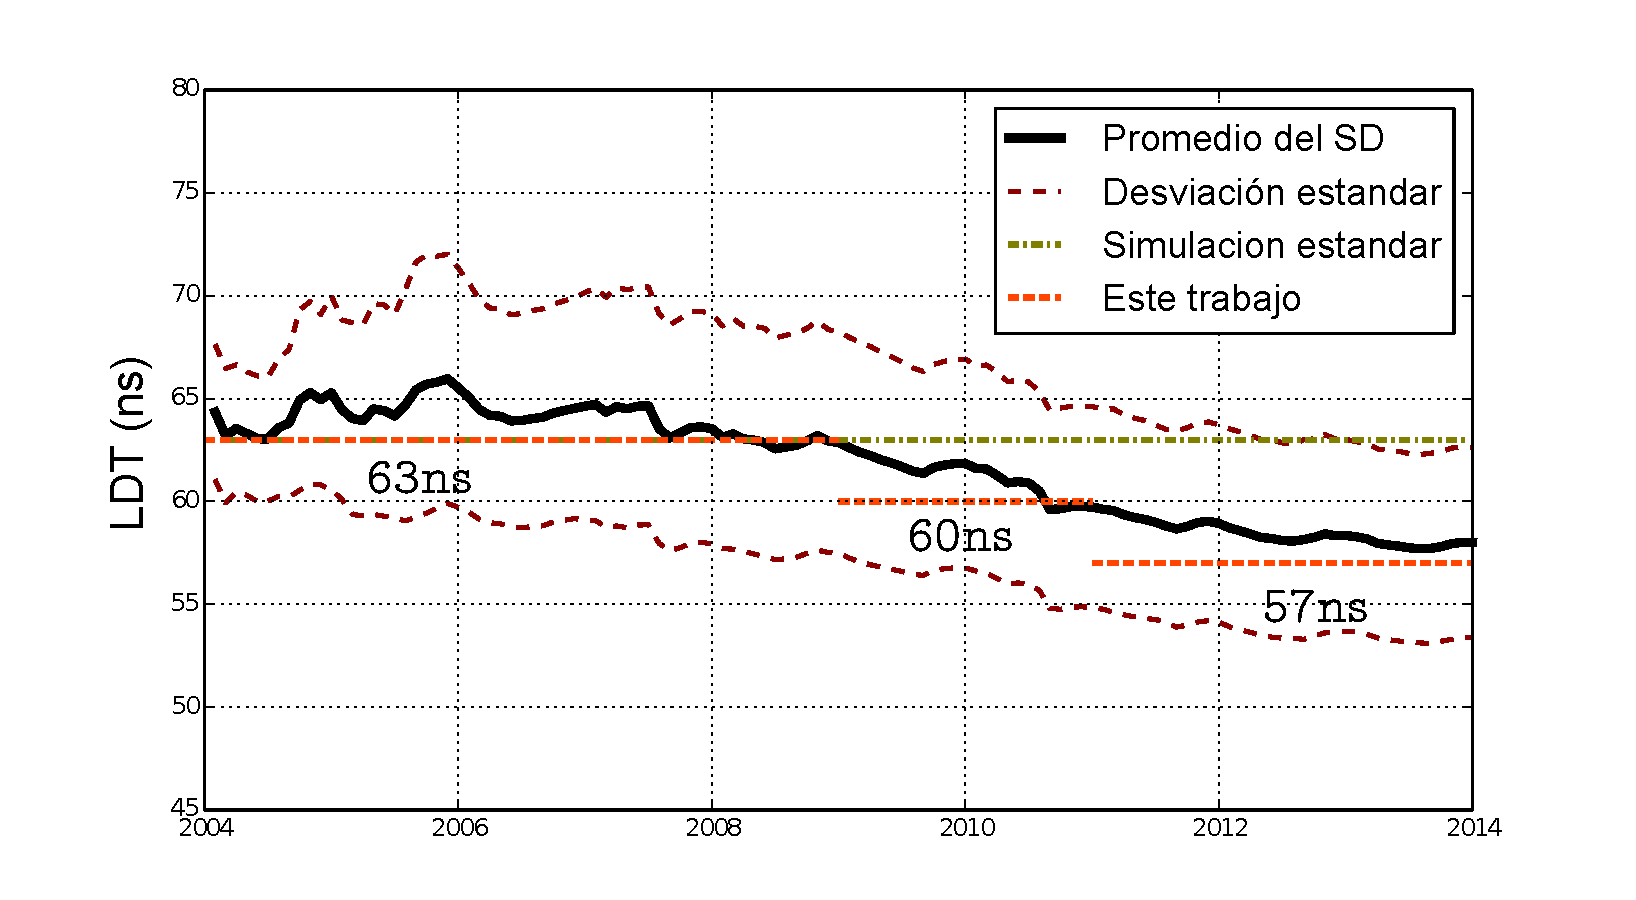
\includegraphics[width=\textwidth]{fig/resultadosAuger/timeEvolution}
			\caption{asd}
			\label{fig:}
		\end{center}
	\end{figure}
	
	\begin{figure}[h!]
		\begin{center}
			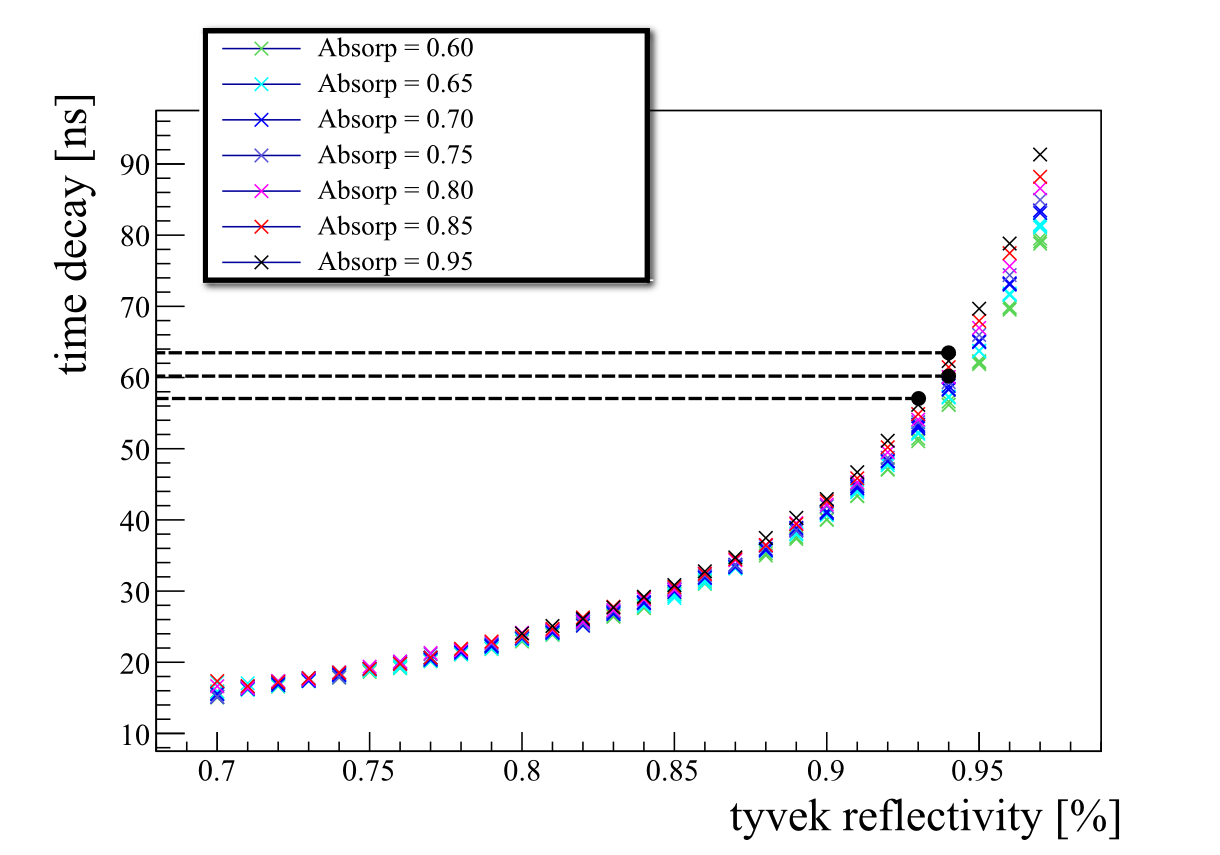
\includegraphics[width=0.9\textwidth]{fig/resultadosAuger/timedecay_vs_reflect_absorp}
			\caption{asd}
			\label{fig:}
		\end{center}
	\end{figure}
	
	\begin{figure}[h!]
		\begin{center}
			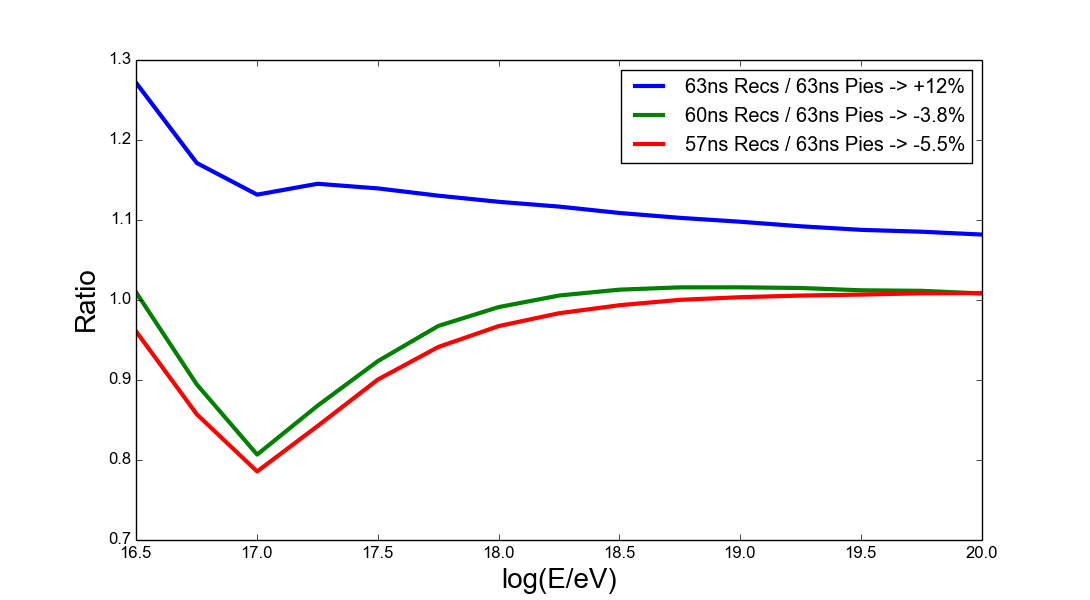
\includegraphics[width=0.9\textwidth]{fig/resultadosAuger/exposure_Arrays}
			\caption{asd}
			\label{fig:}
		\end{center}
	\end{figure}
	
	\begin{table}[h!]
	\centering
	 \begin{tabular}{l|ccc|c|c}
				Period       & tyRef & wAbs & LDT        & Exp Contrib  &   Exp Change \\
				\hline
				$[2004 - 2008]$ & 0.94  & 100  & $\sim63$ns & $33.2\%$     &   $+12\%$ \\
				$[2009 - 2010]$ & 0.94  & 80   & $\sim60$ns & $25.6\%$     &   $-3.8\%$\\
				$[2011 - 2013]$ & 0.93  & 100  & $\sim57$ns & $41.2\%$     &   $-5.5\%$\\
			\end{tabular}
	\end{table}
	
	
\section{Errores sistem\'aticos}
			
	\begin{table}[h!]
	\centering
	\footnotesize
		\begin{tabular}{|c|c|c|c|c|}
		\hline
		Source of  & ES        & DGH       & DGL        & Combined         \\
		systematic & ($90^\circ,95^\circ$) & ($75^\circ,90^\circ$) & ($65^\circ,75^\circ$) & ES / DGH / DGL   \\
		\hline
		& {\tiny \bf GAP 2013-100}     & \multirow{2}{*}{\tiny \bf PRD 84, 2011}    &   \multirow{2}{*}{\tiny \bf GAP2013-013} & \multirow{2}{*}{\tiny \bf 83.9\% / 13.7\% / 2.4\% }\\
		& {\tiny \bf PRD 79, 2009}     &     &  &  \\
		\hline
		
		Int. generator                   	    &  not eval.    &   0\%, -7\%     &   +3\%, -4\%  & +0.07\%, -1.0\% \\
		
		\hline
		
		pdf in generator                &  not eval.    &   0\%, -7\%     &   +4\%, -5\%  & +0.1\%, -1.0\% \\
		
		\hline
		
		EAS simulation	                     	    &  not eval. &   0\%, -17\%    &   +17\%, 0\%  & +0.4\%, -2.3\% \\
		
		\hline
		
		Hadronic model                  		    & +4.7\%, -1\%      &  +5\%, -2\%     &   +0\%, -6\%  & +4.6\%, -1.3\% \\
		
		\hline
		Thinning                                        & +0.3\%, 0\%   &  +7\%,  0\%     &   +7\%,  0\%  & +1.1\%, -0.0\% \\
		\hline
		Detector simulator                              & not eval.     &  not eval.      &   +5\%,  -5\% & +0.1\%, -0.1\% \\
		\hline
		\hline
		{\bf $\bm{ \sigma_{\nu_\tau}\ \otimes\ \tau}$ E-loss}    & \multirow{2}{*}{\textcolor{Red}{+40\%, -33\%}}  & \multirow{2}{*}{+9\%, -9\%}  & \multirow{2}{*}{+7\%, -7\%} & \multirow{2}{*}{\bf +33.6\%, -27.7} \\
		$\sqrt{H^2+I^2}$                                     &                 &                 &             & \\
		\hline
		\hline
% 				%%%%%%%%%%%%%%%%%%%%%%%%%%%%%%%%%%%%%%%%%%%%%%%%%%%%%%%%%%%%%%%%%%%%%%%%%%%%%%%%%%%%%%%%%%%%%%%%%%
		{\bf Topography} 	                            &  +18\%, 0\%    & included & not applicable   & +15.1\%, 0\%  \\

		\hline
		\hline
		{\bf Total}                     &  \multicolumn{3}{c|} {}  & {\bf +37.1\%, -27.9\%}         \\
		\hline
		%%%%%%%%%%%%%%%%%%%%%%%%%%%%%%%%%%%%%%%%%%%%%%%%%%%%%%%%%%%%%%%%%%%%%%%%%%%%%%%%%%%%%%%%%%%%%%%%%%
		\end{tabular}
	\end{table}

\section{Analisis ciego}

	\subsection{Abriendo la caja}
	
	\subsection{L\'imite al flujo difuso y diferencial}
	\begin{figure}[h!]
		\begin{center}
			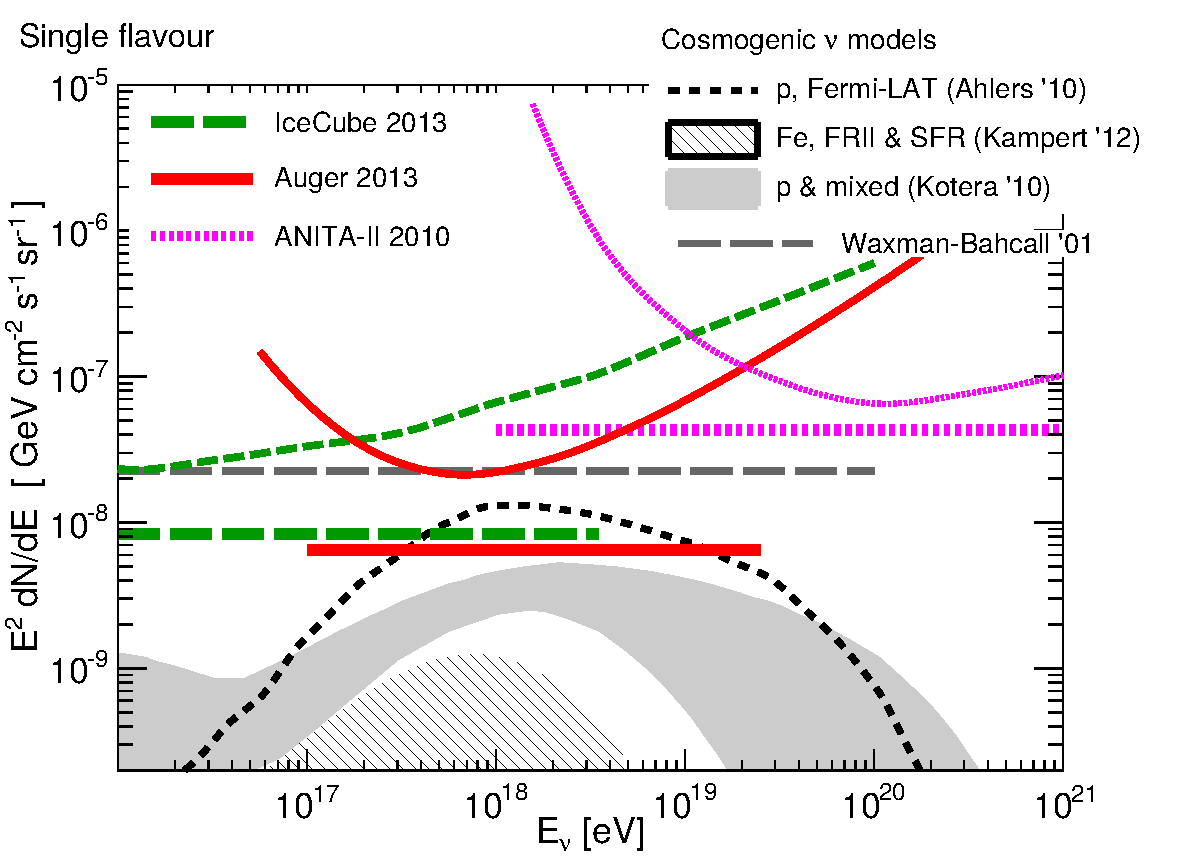
\includegraphics[width=0.9\textwidth]{fig/resultadosAuger/limits_combined_ageing}
			\caption{asd}
			\label{fig:}
		\end{center}
	\end{figure}
	
	\begin{table}[h!]
		\begin{center}
		\renewcommand{\arraystretch}{2.0}
			\begin{tabular}{|c|c|} 
			\hline
			Diffuse flux       &  Expected number of events   \\
			Neutrino Model     &  (1 Jan 04 - 20 Jun 13)   \\
			\hline
			\hline
			Cosmogenic (Kampert {\it et al.}) - proton, FRII      &  \textcolor{Red}{$\sim$ 4.0}  \\
			\hline
			Cosmogenic (Ahlers {\it et al.}) - proton, Fermi-LAT  &  \textcolor{Red}{$\sim$ 3.2}  \\
			\hline
			Cosmogenic (Kampert {\it et al.}) - proton, SFR       &  \textcolor{Blue}{$\sim$ 0.9}  \\
			\hline
			Cosmogenic (Kotera {\it et al.}) - band               &  \textcolor{Blue}{$\sim$ 0.5 $-$ 1.4}  \\
			\hline
			Cosmogenic (Kampert {\it et al.}) - iron, FRII        &  $\sim$ 0.3  \\
			\hline
			\end{tabular}
		\end{center}
	\end{table}
	

	
	\begin{figure}[h!]
		\begin{center}
			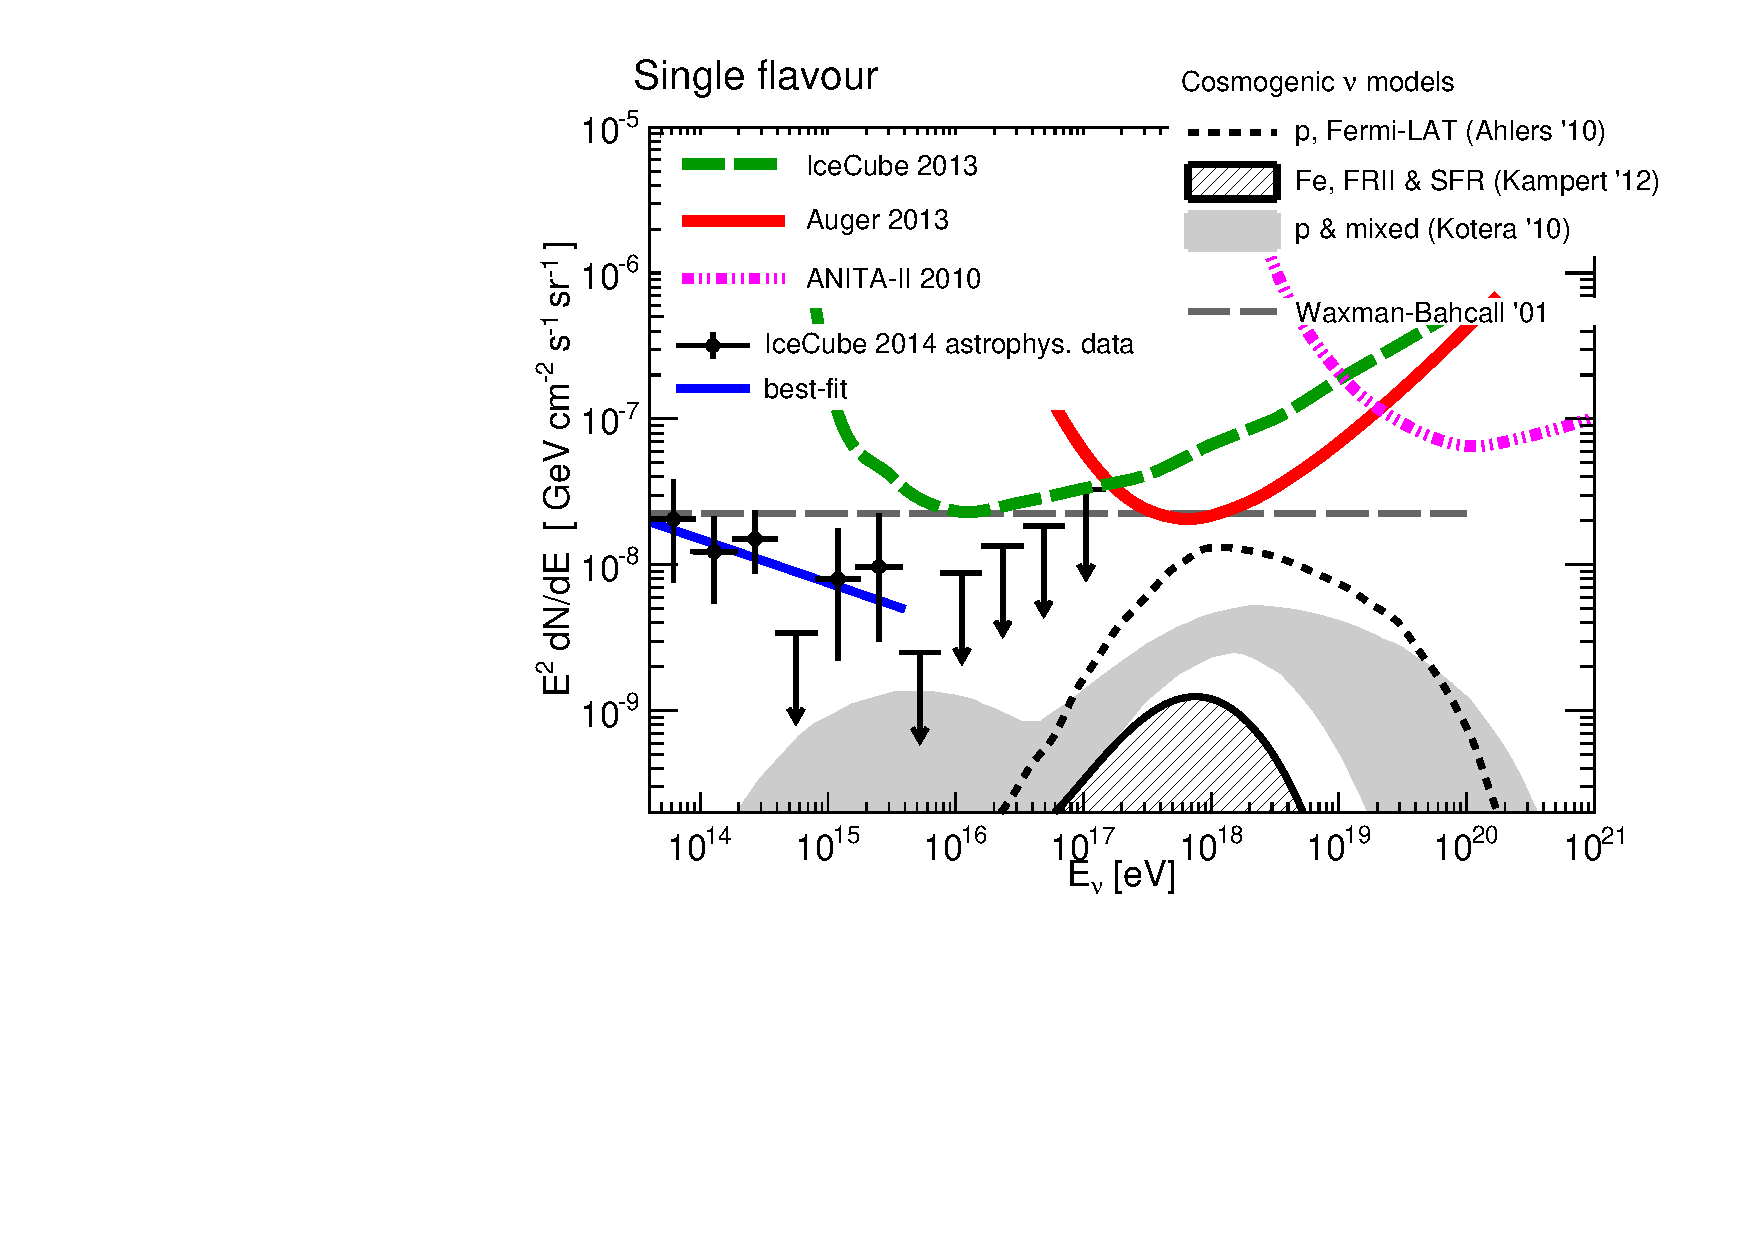
\includegraphics[width=0.9\textwidth]{fig/resultadosAuger/diff_limits_and_many_models_IceCube_data_noextrap}
			\caption{asd}
			\label{fig:}
		\end{center}
	\end{figure}

	
	